	\gls{xml} schema languages are formal languages used to define schemas. A schema represents the definition of the \emph{syntax} and \emph{semantics} that is allowed for an \gls{xml} authoring language \cite{book:moller06}. The syntax consist of defining the vocabulary of the language as well as the different structures in which the elements and attributes are permitted. In contrast, the semantics determines whether or not the syntax expressed in an \gls{xml} document is meaningful. 

	The use of a schema language to formalise an \gls{xml} authoring solution permits obtaining instance specifications that are non-ambiguous and benefits the software program that parses the instances since the number of errors can be reduced or eliminated. In order to check whether an \gls{xml} document conforms to a specific \gls{xml} language, a schema processor, which is an implementation program for an \gls{xml} schema language, takes two arguments: the \gls{xml} document or instance; and the schema (see Figure \ref{fig:background:validationProcess}). This processor, automatically decides the validity of a document and in addition, for those documents that are not valid, it provides a report document explaining the reasons of its failure.

	\begin{figure}[H]
	\centering
	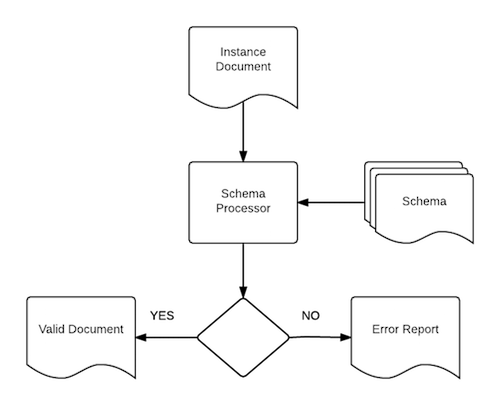
\includegraphics[width=0.75\textwidth]{background/img/validationProcess.png}
	\caption{XML validation process}
	\label{fig:background:validationProcess}
	\end{figure}

	During the process of validating \gls{xml} documents against an \gls{xml} language, four different levels of validation \cite{proc:stuhrenberg10} are checked in order to ensure the correctness of an \gls{xml} specification:
	\begin{enumerate}
		\item \emph{Structure}: This level validates the mark-up introduced as well as the order and occurrences of elements and attributes.
		\item \emph{Data-types}: At this stage it is determined whether the content defined for elements and attributes conforms to the data-types defined in the schema. 
		\item \emph{Integrity constraints}: This level verifies uniqueness of identifiers as well as checks that any reference points to existing keys. Usually, the keys and references to these, are values that are set for attributes.
		\item \emph{Business rules}: At this level, any additional data constraints \cite{proc:vandervlist06} that cannot be categorised in any of the above mentioned levels is checked. This level is very specific to the application domain in which the authoring \gls{xml} language was designed for. 
	\end{enumerate}

	The \gls{xml} schema languages are divided into two approaches: grammar-based and rule-based \cite{stuhrenberg13}. The grammar-based schema languages specify the mark-up, structure and data-types expected for \gls{xml} documents. For instance, they restrict the presence of attributes and elements, the type expected for values, the order in which elements or attributes may appear in the document or the minimum and maximum number of occurrences allowed. In contrast, the rule-based schema languages mainly ensure that the relationships among elements and attributes is consistent. However, they can also constraint \gls{xml} documents by incorporating business specific rules that make specifications meaningful for the application domain.

	Different schema languages exist today aimed to express constraints that are checked at any of the above mentioned validation levels. The three most popular grammar-based schema languages are \gls{dtd}, \gls{xsd} and \gls{relaxng}. Regarding the rule-based language formalisms, \gls{sch} is the only candidate representative. Table \ref{tab:background:schemasTable} summarises the validation levels that these schema languages support. Throughout the next following subsections, the schema languages most relevant to ensure the correctness of \gls{xml} specifications are explored.
	
	\begin{table}[h]
	\centering {\small{}}%
	\begin{tabular}{|c|c|c|c|c|}
	\hline 
	 & \textbf{\small{}DTD}{\small{} } & \textbf{\small{}XSD}{\small{} } & \textbf{\small{}RELAX NG}{\small{} } & \textbf{\small{}SCH}\tabularnewline
	\hline 
	\hline 
	\textbf{\small{}Structures}{\small{} } & {\small{}Basic } & {\small{}Yes } & {\small{}Yes } & {\small{}No}\tabularnewline
	\hline 
	\textbf{\small{}Data-types}{\small{} } & {\small{}Limited } & {\small{}44 built-in } & {\small{}Not directly } & {\small{}Not directly}\tabularnewline
	\hline 
	\multirow{3}{*}{\textbf{\small{}Integrity Constraints}{\small{} }} & ID & {\small{}unique} & \multirow{3}{*}{{\small{}Not directly }} & \multirow{3}{*}{{\small{}Yes}}\tabularnewline
	 & IDREF & key &  & \tabularnewline
	 &  & key-ref &  & \tabularnewline
	\hline 
	\textbf{\small{}Business rules}{\small{} } & {\small{}No } & {\small{}No } & {\small{}No } & {\small{}Yes}\tabularnewline
	\hline 
	\end{tabular}{\small{}\caption{Validation levels supported by the most popular XML schema languages}
	\label{tab:background:schemasTable} }
\end{table}

	\subsection{Document Type Definition (DTD)}\label{sec:background:dtd}

	\gls{dtd} is the built-in schema language since the first working draft of \gls{xml} \cite{web:w3cdtd}. There are many \gls{xml} authoring languages that are specified using \gls{dtd} such as \gls{xhtml} or \gls{triples}. The last mentioned, is known as the standard \gls{xml} language for describing questionnaires. \gls{dtd} has basic support to define syntax for documents since it is not possible to constraint the order and occurrences of elements when character data and elements are allowed within an element structure. Regarding the data-types, it is neither capable of constraining character data (e.g. id attribute for section starts with section followed by any number) nor allows frequent used types such as integer, date or \gls{uri}. In regard to the integrity constraints, it provides ID and IDREF for uniqueness and referential key respectively. However, any defined ID works for the entire document not being able to specify a more restricted scope (e.g. the question id cannot be duplicated across different sections). Moreover, compound keys, i.e. those that combine different attributes to form a key is not supported either. With regards to business rules, there is no mechanism that permits validating semantics over syntactically valid \gls{xml} instances. 

	\gls{dtd} was designed before the name-space mechanism was introduced. This feature, which permits reusing other schema specifications to create a new \gls{xml} language, is not provided and consequently it is not only hard to create modular schemas but also it is difficult to evolve them. Furthermore, a schema defined through \gls{dtd} does not use \gls{xml} notation so checking that a specification of an \gls{xml} language conforms to \gls{dtd} requires the use of non-standard \gls{xml} tools to verify its validity.

	\subsection{XML Schema Definition (XSD)}\label{sec:background:xsd}
	\gls{xsd} is the recommendation schema language for \gls{w3c} \cite{web:w3cxsd}. It was designed to be more expressive than \gls{dtd} and introduces name-spaces, data-types and an \gls{xml} syntax for restricting well-formed \gls{xml} files. As such, it permits importing structures of elements through the \gls{uri} mechanism, uses \gls{xml} syntax to express constraints, which eliminates the need to learn a new proprietary syntax and provides a richer built-in data-types system. Additionally, to strengthen the data-types set, it allows the definition of customised types through restriction (e.g. \gls{url} type is a subset of the string base type) and by extension (e.g. an element single question extends from question element by adding a set of open-closed response elements).

	This schema language unlike its counterparts, provides a better mechanism to express integrity constraints for \gls{xml} documents. \gls{xsd} overcomes the limitations of ID, IDREF that are present in \gls{dtd} by using a subset of XPath Query Language (see Section \ref{sec:background:xPath}) to define unique values for elements or attributes and to reference these through \emph{key} and \emph{key-ref} features respectively. For instance, Listings \ref{code:background:xsd} defines a key to ensure the uniqueness of a question (e.g. intro, single, multiple or open) in the context of a section from a survey through a \emph{selector} element. Moreover, to determine what attribute of a question element is used to check the uniqueness, the \emph{field} element is utilised. Similarly, in that example, the key-ref uses the selector to select a variable within a routing element in which the attribute ref is used to hold the reference to a unique question key. Note that key-ref also defines a refer attribute which points at a key element previously defined in the schema for an authoring language.

	\lstinputlisting[caption={Key and references in XSD},label={code:background:xsd}]{background/xsd_integrity.xml}

	The above mentioned integrity constraints could be used to verify that the document from Listings \ref{code:background:xmlCase} does not actually introduce duplicate keys for question ids neither specifies a reference to a non-existent question id within the routing. 

	\gls{xsd} is one of the most used schema language for defining \gls{xml} languages, mainly because supports enough expressiveness to define structure, data-types and integrity constrains for \gls{xml} documents. However, it is hard to learn due to the amount of features that provide and does not introduce any mechanism to express business rules. \footnote{The version 1.1. introduces assertions to express business rules through a subset of XPath expressions (attributes, children and descendants of an element) \cite{web:w3cxsdassertion}. However other existing relationships among \gls{xml} documents such as parent, ancestors or siblings are unable to express which restrict its expressiveness and usage.}

	\subsection{Regular Expression Language for XML New Generation (RELAX NG)}\label{sec:background:relaxNg}
	%http://www.iso.org/iso/home/store/catalogue_tc/catalogue_detail.htm?csnumber=52348
	\gls{relaxng} is a schema language developed within the \gls{oasis}. This language was built with the design principles of simplicity and expressiveness. As such, its syntax to express constraints for \gls{xml} documents is closer to plain English instructions \cite{book:vandervlist03}. \gls{relaxng} is part of the \gls{iso}/\gls{iec} 19757. Specifically, it is the candidate schema language for describing structure and content of \gls{xml} documents. 

	The data-types and integrity constraints are not directly supported by the language so it relies on external schema languages to address these tasks. Specifically, the data-types for elements and attributes are usually imported from \gls{xsd} whereas the integrity constraints are weakly supported by having a special compatibility data-type library that uses ID and IDREF from \gls{dtd}. Regarding the business rules, as this language is categorised as grammar-based, it does not directly offers features for specifying additional constraints.

	\subsection{Schematron (SCH)}\label{sec:background:sch}
	%http://www.iso.org/iso/home/store/catalogue_tc/catalogue_detail.htm?csnumber=55982
	\gls{sch} is a schema language designed by Rick Jelliffe \cite{web:doodds01}. This language differs from grammar-based \gls{xml} schema languages in that it is rules-based, i.e. defines assertions within a rule context that are evaluated over \gls{xml} instance documents. This language, likewise \gls{relaxng}, also takes part from the \gls{iso}/\gls{iec} 19757 and constitutes the standard reference to ensure that documents match the rules defined through a schema. In \gls{sch}, the constraints are specified via XPath query language (see Section \ref{sec:background:xPath}). The use of these expressive queries, permits defining any kind of tree relationships (e.g. child, parent, ancestor) that are inherited in \gls{xml} documents making this schema language unique in terms of expressing semantics.

	The core constructs of Schematron are patterns, rules and assertions. Listings \ref{code:background:schematron} describes an integrity constraint that check the uniqueness of section identifiers. The pattern element is used to group different rules. A rule requires a context attribute which constitutes the path used to evaluate one or more asserts (e.g. this rule is fired for every section within the survey element). An assert is specified through the test attribute and addressed to check a constraint within the context rule described. For instance, the assert example counts the preceding section's identifiers that are equals to the identifier set through the place holder \$id (e.g. let element) in order to determine whether is zero or not. A false result for the assert, displays the customised message within that element.  
	\lstinputlisting[caption={Integrity constraint expressed in SCH},label={code:background:schematron}]{background/sch_integrity.xml}

	The validation of \gls{xml} documents against a \gls{sch} schema can be carried out either by using an \gls{xslt} \cite{web:w3cxslt} processor or by using an XPath implementation. The \gls{xslt} approach, represented in Figure \ref{fig:background:sch_xslt_processor} requires performing two steps:

	\begin{figure}[H]
	\centering
	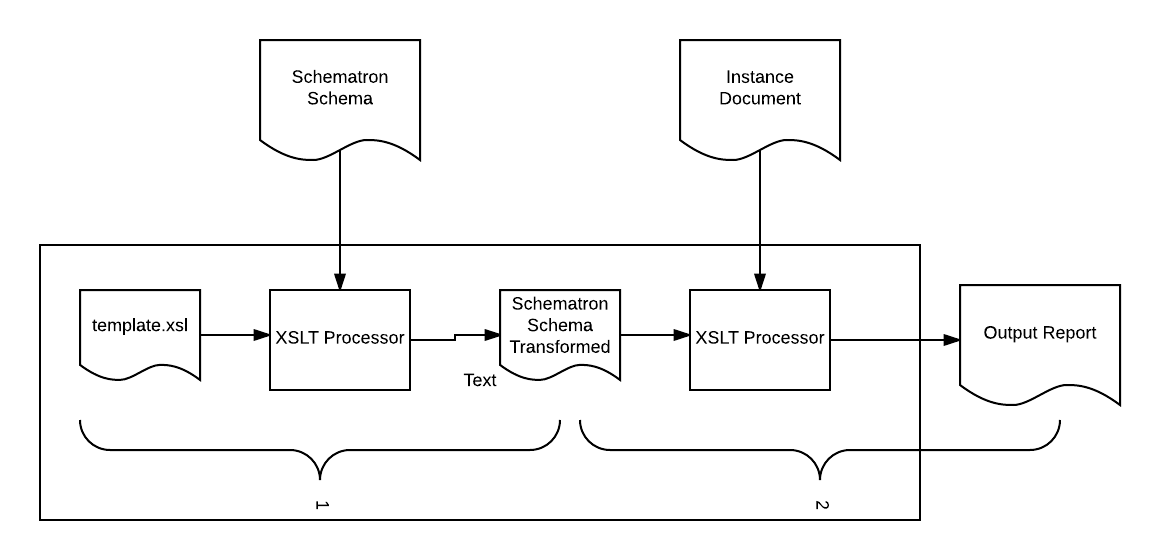
\includegraphics[width=0.90\textwidth]{background/img/sch_xslt_processor.png}
	\caption{Schematron XSLT validation process}
	\label{fig:background:sch_xslt_processor}
	\end{figure}

	\begin{itemize}
		\item First, an \gls{xslt} processor gets a \gls{sch} schema together with a pre-defined \gls{sch} template, provided by Academia Sinica Computing Centre \footnote{\url{https://www.ascc.sinica.edu.tw/en/about/overview.html}}, in order to produce a transformed \gls{sch} schema understandable by the \gls{xslt} processor.
		\item Second, the transformed schema, together with the \gls{xml} document is passed to the \gls{xslt} processor to finally produce the output report based on the rules and assertions in the original \gls{sch} schema defined.
	\end{itemize}

	The XPath implementation, unlike its counterpart, is faster for validating \gls{xml} documents since the transformation step is not needed. However, it has less functionality due to \gls{xslt}-specific functions such as document() or key() which are not supported. For instance, \emph{document} function permits validating rules among \gls{xml} documents.

	The high expressiveness of \gls{sch} not only makes this schema language the best for representing any integrity constraint \cite{art:murata05} but also extends its capacity to define any sort of business rule. Regarding the structure, although it is able to describe many instances of grammars \cite{web:jellife07}, this constraining level is best addressed through grammar-based languages. In regard to the data-types, \gls{sch} does not directly provide any built-in type. However, these may be simulated using the XPath functions.